\documentclass{article}

\usepackage{fancyhdr}
\usepackage[a4paper, hmargin=1in,vmargin=1.5in]{geometry}
\usepackage{xcolor}
\usepackage{amsmath}
\usepackage{amsthm}
\usepackage{amssymb}
\usepackage{amsfonts}
\usepackage[parfill]{parskip}
\usepackage{hyperref}
\usepackage{url}
\usepackage{floatrow}
\usepackage{graphicx}

\pagestyle{fancy}
\fancyhf{}
\lhead{Assignment 2}
\rhead{Question \thesection}
\lfoot{Group 13}
\rfoot{Page \thepage}
\renewcommand{\footrulewidth}{1pt}
\newtheorem*{remark}{Remark}
\begin{document}
\title{EE 325 Group 13 - Assignment 2 }
\author{
	Manideep Vudayagiri\\
	\textbf{190070074}
	\and
	Shreyas Nadkarni\\
	\textbf{19D170029}
	\and
	Tarun Kumar\\
	\textbf{19D070062}
	\and
	Ashish Pol\\
	\textbf{190070011}
	\and
	Rohit Ahirwar\\
	\textbf{190070053}
	
	
}

\maketitle
\tableofcontents
\thispagestyle{empty}
\clearpage
\pagenumbering{arabic}

\newpage

\section{Question 1 - (2-5)}
\label{Q1}
\textbf{2-5} Prove and generalize the following identity : \\
\begin{equation*}
	P(A \cup B \cup C) = P(A) + P(B) + P(C) - P(AB) - P(AC) - P(BC) + P(ABC)
\end{equation*}

\hspace{1em} \large{\textbf{SOLUTION :}} \\
We will use the following equation for the proof :
\begin{equation}
\label{(1)}
	P(A \cup B ) = P(A) + P(B) - P(AB)
\end{equation}
\begin{proof}
	Since $A \cup B \cup C = (A \cup B) \cup C$,  using \ref{(1)}, we can say that : \\ 
	\begin{align*}
	    P(A \cup B \cup C) &=P((A \cup B) \cup C) \\
	    &= P(A \cup B) + P(C) - P((A \cup B) \cap C)) \\ &\text{(using \ref{(1)})} \\
	    &= P(A) + P(B) + P(C) - P(AB) - P((A \cup B) \cap C)) \\ &\text{(using \ref{(1)})} \\
	    &= P(A) + P(B) + P(C) - P(AB) - P((A \cap C) \cup (B \cap C)) \\ &\text{(using distributive property of $\cap$ and $\cup$)} \\
	    &= P(A) + P(B) + P(C) - P(AB) - ((P(A \cap C) + P(B \cap C) - \\ &P((A \cap C) \cap (B \cap C))) \text{  (using \ref{(1)})} \\
	    &= P(A) + P(B) + P(C) - P(AB) - P(AC) - P(BC) + P(ABC) \\
	    & \text{Since }  (A \cap C) \cap (B \cap C) \equiv A \cap B \cap C  \text{(using distributive property of $\cap$)} 	
	 \end{align*}
\end{proof}

For the General formula we shall use induction on $n$(Total number of events) : \\
\\
\textbf{Claim :}  \\
$$ P(A_1 \cup A_2 \dots A_n) = \sum_{i=1}^{n}P(A_i)  -  \sum_{\substack{i,j =1 \\ i \neq j}}^{n}P(A_i A_j)  +  \sum_{\substack{i,j,k = 1 \\ i \neq j \neq k}}^{n}P(A_i A_j A_k)  +  \dots   (-1)^{n+1}P(A_1 A_2 \dots A_n)$$
\begin{proof}
	We shall prove the above claim using induction on $n$ \\
	For the base case of $n = 1$, \\
	$P(A_1) = P(A_1)$
	Which is trivially true. \\
	For the inductive step, let $n > 1 and$ assume (the inductive hypothesis) for $n-1$ : \\
	\begin{equation}
	\label{(2)}
	P(A_1 \cup A_2 \dots A_{n-1}) = \sum_{i=1}^{n-1}P(A_i) - \sum_{\substack{i,j =1 \\ i \neq j}}^{n-1}P(A_i A_j) + \sum_{\substack{i,j,k = 1  \\ i \neq j \neq k}}^{n-1}P(A_i A_j A_k) + \dots   (-1)^{n}P(A_1 A_2 \dots A_{n-1})
	\end{equation}
	Now we can apply the equation of union of two sets to the two events $A_n$ and $(A_1 \cup A_2 \dots A_{n-1})$ to deduce that : \\
	
	$$P((A_1 \cup A_2 \dots A_{n-1}) \cup A_n) = P(A_1 \cup A_2 \dots A_{n-1}) + P(A_n) - P((A_1 \cup A_2 \dots A_{n-1}) \cap A_n) \text{(using \ref{(1)})}$$
	$$= \Big(\sum_{i=1}^{n-1}P(A_i) - \sum_{\substack{i,j =1 \\ i \neq j}}^{n-1}P(A_i A_j) + \sum_{\substack{i,j,k = 1  \\ i \neq j \neq k}}^{n-1}P(A_i A_j A_k) + \dots   (-1)^{n}P(A_1 A_2 \dots A_{n-1})\Big) + P(A_n)$$ \\  $   - P((A_1 \cup A_2 \dots A_{n-1}) \cap A_n) $  (using \ref{(2)})\\
	$$= \Big(\sum_{i=1}^{n-1}P(A_i) - \sum_{\substack{i,j =1 \\ i \neq j}}^{n-1}P(A_i A_j) + \sum_{\substack{i,j,k = 1  \\ i \neq j \neq k}}^{n-1}P(A_i A_j A_k) + \dots   (-1)^{n}P(A_1 A_2 \dots A_{n-1})\Big) + P(A_n)$$ \\  $   - P((A_1 \cap A_n) \cup (A_2 \cap A_n) \cup \dots (A_{n-1} \cap A_n)) \text{(using distributive property of $\cap$ and $\cup$)}$ \\
	$$= \Big(\sum_{i=1}^{n-1}P(A_i) - \sum_{\substack{i,j =1 \\ i \neq j}}^{n-1}P(A_i A_j) + \sum_{\substack{i,j,k = 1  \\ i \neq j \neq k}}^{n-1}P(A_i A_j A_k) + \dots   (-1)^{n}P(A_1 A_2 \dots A_{n-1})\Big) + P(A_n)$$ \\  $$   - \Big(\sum_{i=1}^{n-1}P(A_i  A_n) + \sum_{\substack{i,j =1 \\ i \neq j}}^{n-1}P(A_i A_j A_n) + \sum_{\substack{i,j,k = 1  \\ i \neq j \neq k}}^{n-1}P(A_i A_j A_k A_n) + \dots (-1)^{n}P(A_1 A_2 \dots A_{n-1} A_n)\Big)$$\\  (using \ref{(2)})\\
	$$ =\sum_{i=1}^{n}P(A_i)  -  \sum_{\substack{i,j =1 \\ i \neq j}}^{n}P(A_i A_j)  +  \sum_{\substack{i,j,k = 1 \\ i \neq j \neq k}}^{n}P(A_i A_j A_k)  +  \dots   (-1)^{n+1}P(A_1 A_2 \dots A_n) $$
		
where in the last line we have used the inductive hypothesis. This completes the proof by induction.
\end{proof}
\section{Question 2 - (2-10)}
\label{Q2}
\textbf{2-10} \textit{(Chain rule)} Show that  : \\
\begin{equation*}
	P(A_n \dots A_1) = P(A_n \mid A_{n-1} \dots A_1) \dots P(A_2 \mid A_1)P(A_1)
\end{equation*}

\hspace{1em} \large{\textbf{SOLUTION :}} \\
\textbf{Definition of Conditional Probability :}\\
For events A,B in the same probability space, such that $Pr(B) > 0$, the conditional probability of A given B is : \\
$$P(A \mid B) = \frac{P(A \cap B)}{P(B)} ,
P(A \cap B) = P(A \mid B) \times P(B) $$

 
We shall prove this by induction on $n$ (number of events)\\
So, for the first case $ n = 1 $ \\
$$P(A_1) = P(A_1)$$
Which is trivially true. \\
For the inductive step, let $n > 1 and$ assume (the inductive hypothesis) that : \\
$$P(A_1 \cap A_2 \dots A_{n-1}) = P(A_1) \times P(A_2 \mid A_1) \times \dots P(A_{n-1} \mid (A_1) \cap (A_2) \dots (A_{n-2})) $$ \\
Now we can apply the definition of conditional probability to the two events $A_n$ and $(A_1 \cap A_2 \dots A_{n-1})$ to deduce that : \\
\begin{align*}
	P(A_n \cap A_{n-1} \dots A_1) &= P((A_n) \cap (A_1 \cap A_2 \dots A_{n-1})) \\
	&= P(A_n \mid (A_1 \cap A_2 \dots A_{n-1})) \times P(A_1 \cap A_2 \dots A_{n-1}) \\
	&= P(A_n \mid (A_1 \cap A_2 \dots A_{n-1})) \times P(A_1) \times P(A_2 \mid A_1) \\ &\times \dots P(A_{n-1} \mid (A_1) \cap (A_2) \dots (A_{n-2})) 
\end{align*}
where in the last line we have used the inductive hypothesis. This completes the proof by induction.

\section{Question 3 - (2-14)}
\label{Q3}
\textbf{2-14}  The events $A$ and $B$ are mutually exclusive. Can they be independent?  : \\

\hspace{1em} \large{\textbf{SOLUTION :}} \\

\textbf{Definition : Independent Events} \\
Events $A$ and $B$ are independent if and only if \\
$$P(A \cap B) = P(A) P(B)  $$

\textbf{Definition : Mutually Exclusive Events} \\
Events $A$ and $B$ are Mutually Exclusive if and only if \\
$$P(A \cap B) = 0  $$

$P(A \cap B) = P(A) P(B)  $ and $P(A \cap B) = 0  $ if and only if $P(A) = 0$ or $P(B) = 0$

Hence, if $A$ and $B$ are mutually exclusive events, they are independent if and only if $P(A) = 0$ or $P(B) = 0$.
\section{Question 4 - (2-16)}
\label{Q4}
\textbf{2-16}  A box contains $n$ identical balls numbered 1 through $n$. Suppose $k$ balls are drawn in succession. (a) What is the probability that $m$ is the largest number drawn? (b) What is the probability that the largest number drawn is less than or equal to $m$?  : \\

\hspace{1em} \large{\textbf{SOLUTION :}} \\
This is an example of sampling without replacement and without ordering. Let $N$ be the total number of possible outcomes, which is equal to the number of ways in which we can select $k$ out of $n$ balls. Therefore,
\begin{equation*}
    N\ = \ {n \choose k }
\end{equation*}
Now, for $m$ to be the largest number picked (call this event $A_m$), the ball numbered $m$ must be one of the $k$ balls drawn and the other $k-1$ balls should come from the first $m-1$ balls. So, if $N_{A_m}$ represents number of favourable outcomes for event $A$,
\begin{equation*}
    N_{A_m}\ =\ {m-1 \choose k-1}
\end{equation*}
So, we get:
\begin{equation*}
\begin{split}
Pr(A_m) & = \frac{N_{A_m}}{N} \\
 & = \frac{{m-1 \choose k-1}}{{n \choose k }} 
\end{split}
\end{equation*}
Now if $B$ represents the event that the largest number drawn is less than or equal to $m$, we have
\begin{equation*}
\begin{split}
    Pr(B) & =\ \sum_{i=k}^{m} P(A_i) \\
            &=\ \sum_{i=k}^{m} \frac{{i-1 \choose k-1}}{{n \choose k}} \\
            &=\ \frac{{k-1 \choose k-1} + {k \choose k-1} + \dots + {m-1 \choose k-1}}{{n \choose k}} \\
            &=\ \frac{{m \choose k }}{{n \choose k}}
\end{split}
\end{equation*}
We summed up the expression in the second last step by writing ${k-1 \choose k-1}$ as ${k \choose k}$ (since both are equal to 1) and then applying the reduction formula: ${n \choose r}\ +\ {n \choose r-1}\ =\ {n+1 \choose r}$ repetitively.

\section{Question 5 - (2-17)}
\label{Q5}
\textbf{2-17}  Suppose $k$ identical boxes contain $n$ balls numbered 1 through $n$. One ball is drawn from each box. What is the probability that $m$ is the largest number drawn?  : \\

\hspace{1em} \large{\textbf{SOLUTION :}} \\
Let $A$ be the event that the largest number drawn is $m$, and $B$ be the event that each number drawn is less than or equal to $m$. We need to find $P(A)$. The event $B$ is an intersection on $k$ independent events, the $i^{th}$ event being that the number drawn from $i^{th}$ box is less than or equal to $m$, and the probability of this event is simply $\frac{m}{n}$. Thus we get,
\begin{equation*}
    Pr(B)\ =\ \Big(\frac{m}{n}\Big)^k
\end{equation*}
\subsection*{Method 1}
Clearly, $Pr(A\ |\ \overline{B})\ =\ 0$. For $Pr(A|B)$, there are $k$ numbers drawn and each belongs to $[1,m]$ so total number of possible outcomes $N\ =\ m^k$. The outcomes where no $m$ has been drawn are unfavourable, and those are $\overline{N}\ = (m-1)^k$. So we get number of favourable outcomes $N_{A|B}\ =\ N\ -\ \overline{N_{A|B}}\ =\ m^k\ -\ (m-1)^k$. Hence, 
\begin{equation*}
    Pr(A|B)\ = \ \frac{m^k\ -\ (m-1)^k}{m^k}
\end{equation*}
So, by the Total Probability Law,
\begin{equation*}
\begin{split}
Pr(A)\ &= \ Pr(A|B)Pr(B)\ +\ Pr(A|\overline{B})Pr(\overline{B}) \\
       &= \ \frac{m^k\ -\ (m-1)^k}{m^k} \times \Big(\frac{m}{n}\Big)^k \\
       &= \ \frac{m^k\ -\ (m-1)^k}{n^k}
\end{split}
\end{equation*}

\subsection*{Method 2}
We notice that event $A$ is a subset of event $B$. So $B\ = A\ + B\overline{A}$, where $A$ and $B\overline{A}$ are mutually exclusive events. 
Also for $B\overline{A}$, we need $k$ balls to be chosen, with the number of each being less than $m$, i.e. from $[1,m-1]$ and total possible outcomes are $n^k$ as before. So,
\begin{equation*}
    Pr(B\overline{A})\ =\ \frac{(m-1)^k}{n^k}
\end{equation*}
Since $A$ and $B\overline{A}$ are mutually exclusive and exhaustive parts of $B$, we have
\begin{equation*}
    Pr(B)\ =\ Pr(B\overline{A})\ +\ Pr(A)
\end{equation*}
\begin{equation*}
    \begin{split}
        Pr(A) &=\ Pr(B)\ -\ Pr(B\overline{A}) \\
              &=\ \Big(\frac{m}{n}\Big)^k\ -\ \frac{(m-1)^k}{n^k} \\
              &=\ \frac{m^k\ -\ (m-1)^k}{n^k}
    \end{split}
\end{equation*}

\section{Question 6 - (2-19)}
\label{Q6}
\textbf{2-19} A box contains $m$ white and $n$ black balls. Suppose k balls are drawn. Find the probability of drawing at least one white ball.  : \\

\hspace{1em} \large{\textbf{SOLUTION :}} \\
Let us find the probability that none of the $k$ balls drawn is white (call this event $\overline{A}$). We want to find $Pr(A)$. There are total $m+n$ balls out of which $k$ are drawn. So total number of possible outcomes = ${ m+n \choose k}$. For no ball to be white, we need each ball to  come from the $n$ black balls. So, number of favourable outcomes (for $\overline{A}$)\ =\ ${ n \choose k}$. Thus,
\begin{equation*}
    Pr(\overline{A})\ =\ \frac{{n \choose k}}{{m+n \choose k}}
\end{equation*}
And thus, 
\begin{equation*}
    Pr(A)\ =\ 1\ -\ \frac{{n \choose k}}{{m+n \choose k}}
\end{equation*}

\section{Question 7 - (2-24)}
\label{Q7}
\textbf{2-24}  Box 1 contains 1000 bulbs of which 10\% are defective. Box 2 contains 2000 bulbs of which 5\% are defective. Two bulbs are picked from a randomly selected box. (a) Find the probability that both bulbs are defective. (b) Assuming that both are defective, find the probability that they came from box 1.  : \\

\hspace{1em} \large{\textbf{SOLUTION :}} \\
Let $B_i$ be the event that the box chosen is box $i$. So we have $B_2 \equiv \overline{B_1}$ and $P(B_1)\ =\ P(B_2)\ =\ 0.5$. Let $D_i$ be the event that the $i^{th}$ bulb is defective and for simplicity let $D\ =\  D_1D_2$ that is the event that both bulbs selected are defective. According to the given data, 100 bulbs in box $1$ and 100 bulbs in box $2$ are defective. Therefore,
\begin{equation*}
    P(D_1|B_1)=\frac{100}{1000}= 0.1,\ \ P(D_2|B_1,D_1) = \frac{99}{999} = \frac{11}{111}
\end{equation*}
So we get
\begin{equation*}
    \begin{split}
        P(D|B_1)\ &=\ P(D_1 D_2|B_1)\\
                 &=\ P(D_1|B_1)\ \times\ P(D_2|B_1,D_1)\\
                 &=\ 0.1\ \times \frac{11}{111}\\
                 &=\ 0.00991\\
    \end{split}
\end{equation*}
Similarly, we get
\begin{equation*}
    \begin{split}
        P(D|B_2)\ &=\ \frac{100}{2000}\ \times \frac{99}{1999}\\
                  &=\ 0.00248\\
    \end{split}
\end{equation*}
\textbf{a)} We want to find $P(D)$. Since $B_1$ and $B_2$ are complements of each other, we can use the total probability rule as follows:
\begin{equation*}
    \begin{split}
        P(D)\ &=\ P(D_1|B_1)P(B_1)\ +\ P(D_1|B_2)P(B_2)\\
              &=\ 0.00991 \times 0.5\ +\ 0.00248 \times 0.5\\
              &=\ 0.00620
    \end{split} 
\end{equation*}

\textbf{b)} Here, we need to find $P(B_1|D)$. Using Bayes Theorem.
\begin{equation*}
    \begin{split}
        P(B_1|D)\ &=\ \frac{P(D|B_1)P(B_1)}{P(D)} \\
              &=\ \frac{0.00991}{0.00620}\\
              &=\ 0.80
    \end{split} 
\end{equation*}

\section{Question 8 - (2-25)}
\label{Q8}
\textbf{2-25} A train and a bus arrive at the station at random between 9 A.M. and 10 A.M. The train stops for 10 minutes and the bus for $x$ minutes. Find $x$ so that the probability that the bus and the train will meet equals 0.5. : \\

\hspace{1em} \large{\textbf{SOLUTION :}} \\
    For the train and bus to meet, one of them should
arrive at the station at a point in the time interval in which the other one is stopped at the station.

Let, $t_B$ and $t_T$ be the times(in minutes) at which the bus and train arrive at the station relative to the 1 hour time interval.

We'll define the events at which they meet as following:\\
$T : \{t_T < t_B < t_T+10 | \{t_T,t_B\}\in(0,60)\} \text{ is the event in which the train arrives first.}\\
B : \{t_B < t_T < t_B+x | \{t_T,t_B\}\in(0,60)\}$ is the event in which the bus arrives first.\\
The event that the bus and train meet at the station is $T\cup B$.\\

$T$ and $B$ are clearly mutually exclusive. Therefore,\\
$$P(T\cup B) = P(T) + P(B)$$

We can plot a graph with $t_T$ on $x-axis$ and $t_B$ on $y-axis$ and find the regions which satisfy $T$ and $B$.
\begin{figure}[H]
    \centering
    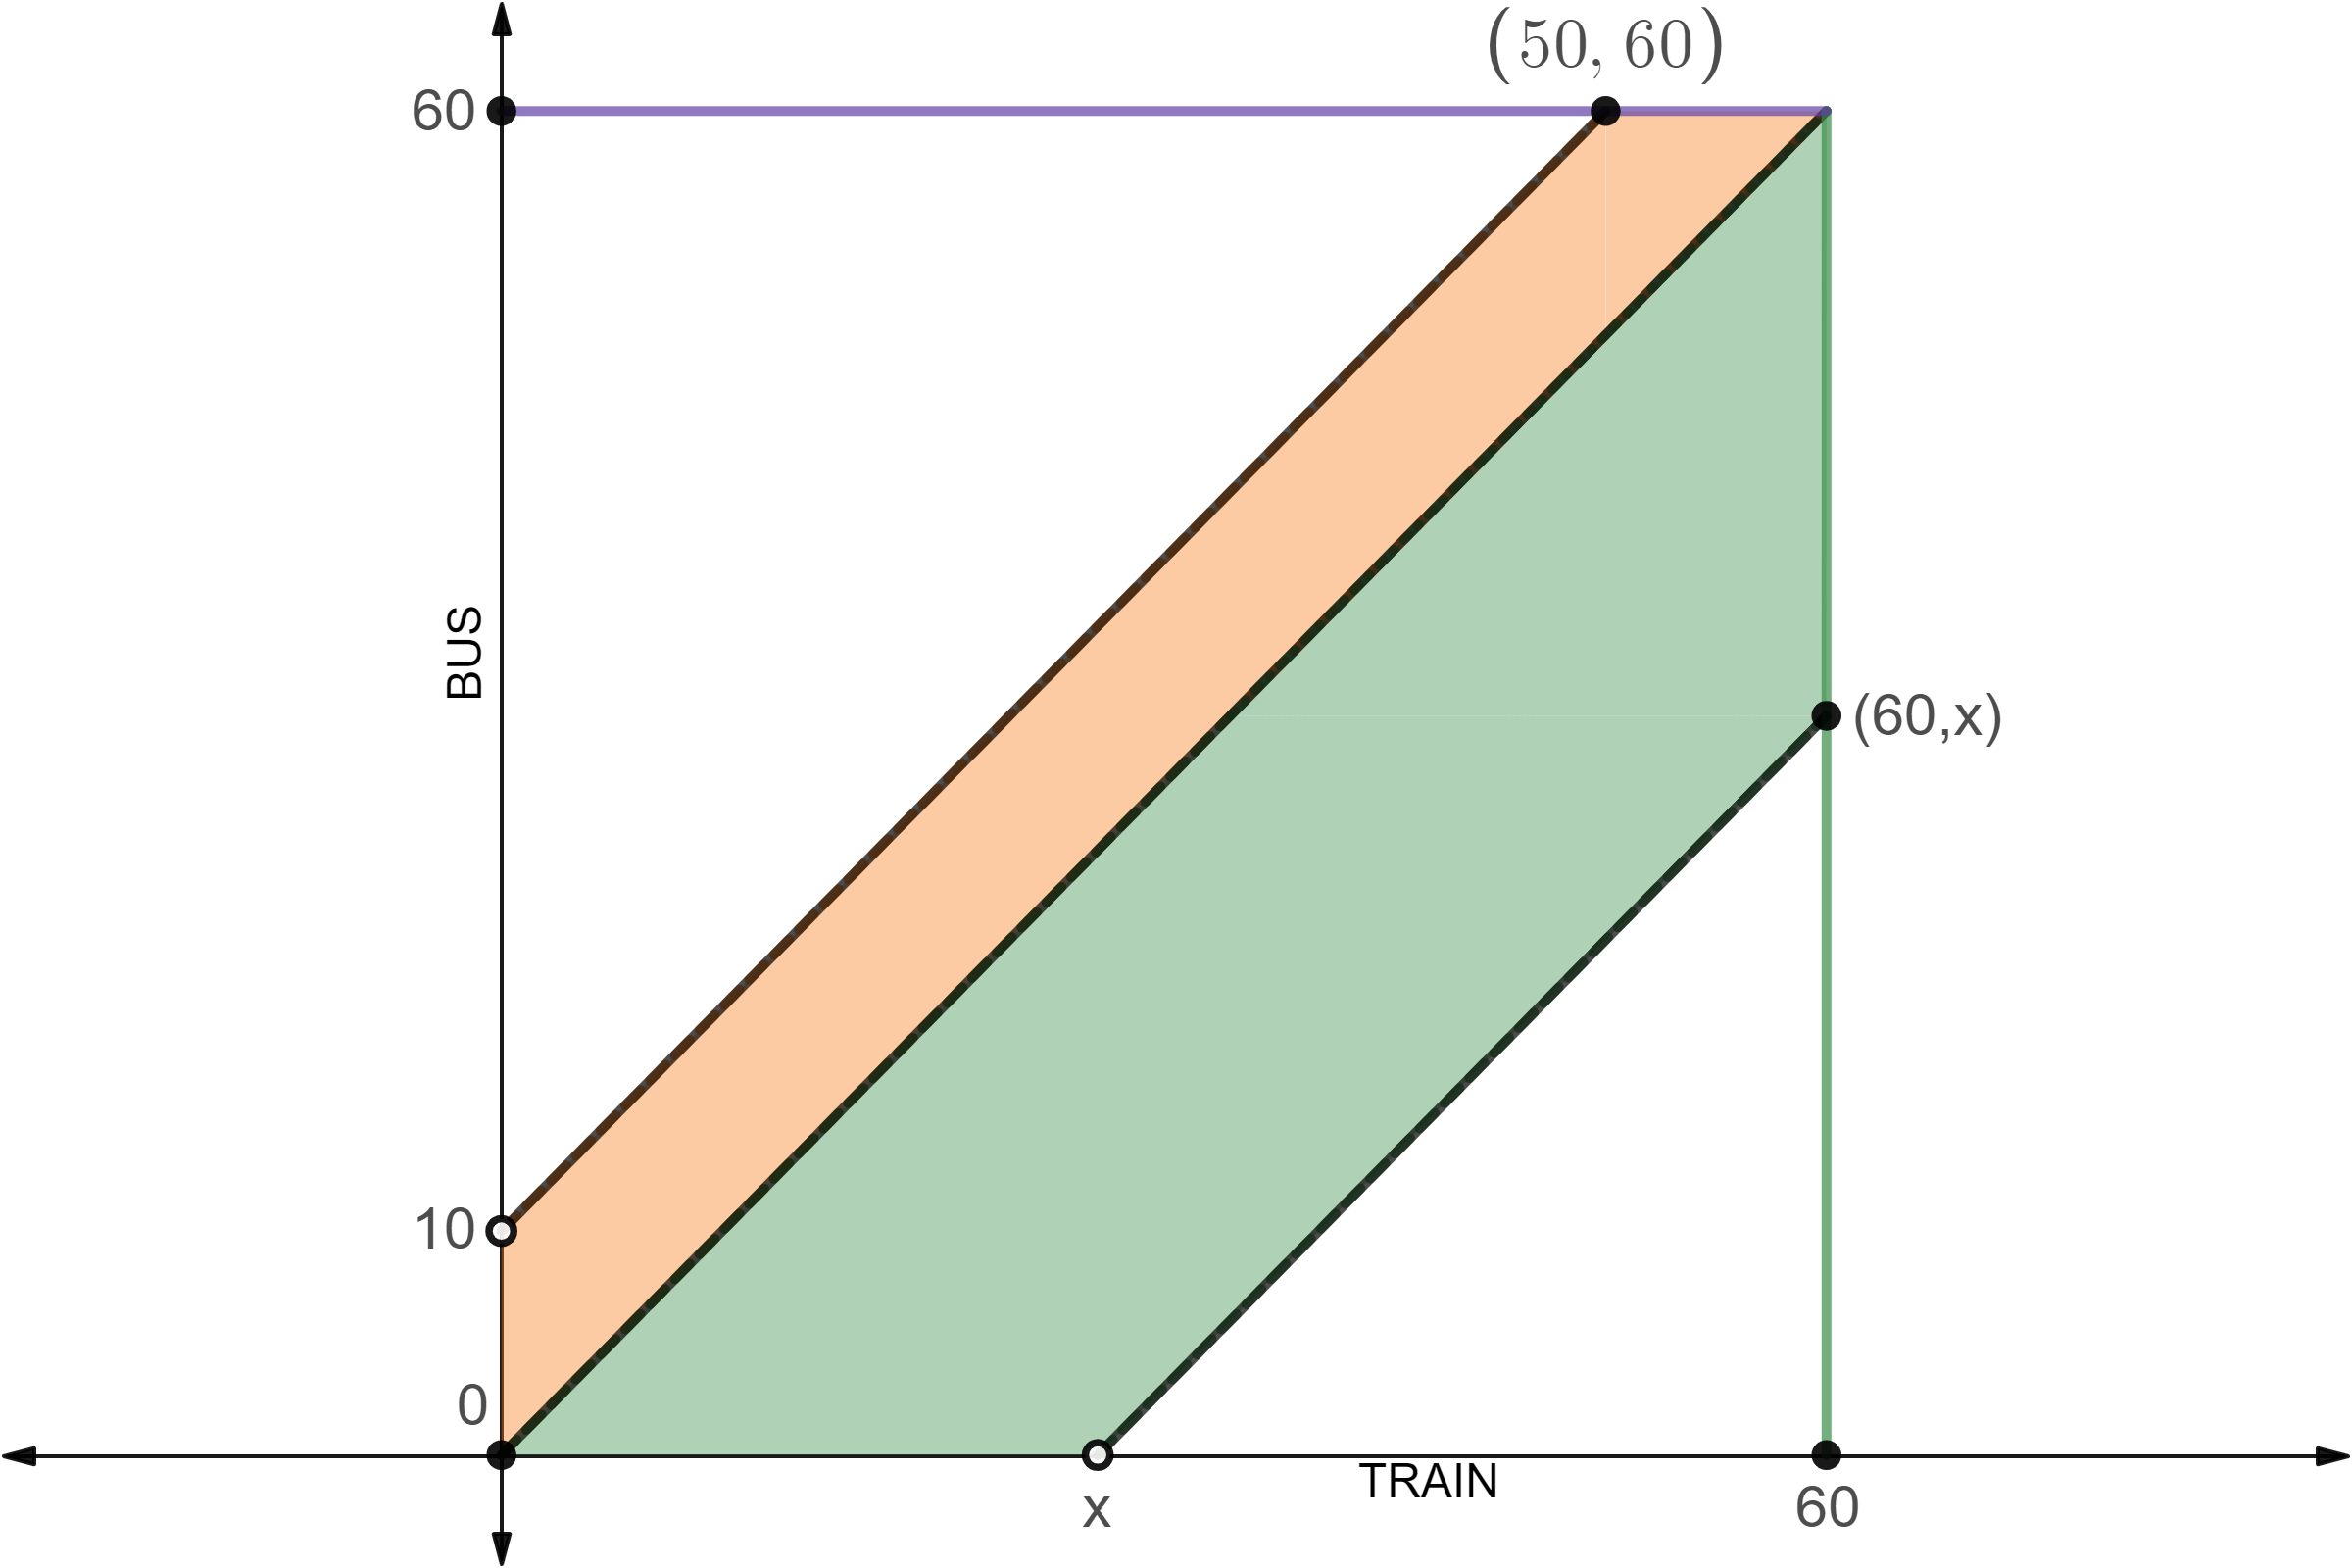
\includegraphics[width=0.8\linewidth]{pics/bustrain.png}
    \caption{Time of arrival at the station: train v/s bus}
    \label{fig:my_label}
\end{figure}
    $$P(T\cup B) = \frac{\text{Area of shaded region}}{\text{Area of the } 60 \times 60 \text{ square region}}$$\\
\begin{align*}
    P(T\cup B) &= \frac{60\times 60 - \Big(\dfrac{(50-0)(60-10)}{2}+\dfrac{(60-x)(x)}{2}\Big)}{60\times 60}\\
    &=\frac{x^2 - 120x + 6100}{7200}
\end{align*}

We need this expression to be equal to 1/2\\
\begin{align*}
    &\Rightarrow \frac{x^2 - 120x + 6100}{7200}=\frac{1}{2}\\
&\Rightarrow x^2 - 120x + 2500 = 0\\
\end{align*}
Solve to get:
$$x = (60 - 10\sqrt{11})$$ 
\section{Question 9 - (2-27)}
\label{Q9}
\textbf{2-27} We have two coins; the first is fair and the second two-headed. We pick one of the coins at random, we toss it twice and heads shows both times. Find the probability that the coin picked is fair.  : \\

\hspace{1em} \large{\textbf{SOLUTION :}} \\
In this experiment we have 8 outcomes. Each outcome is a selection of a particular coin and a specific sequence of heads or tails. For example, $FNN$ corresponds to selecting the fair coin followed by getting two heads. Let $F$ be the event that the selected coin is fair. So, given $F$ happens, we will have four possible outcomes: $FHH,\ FHT,\ FTH,$ and $FTT$. If $\overline{F}$ happens then we have only one outcome: $\overline{F}HH$, since the other coin is two headed. So, we have the following quantities:
\begin{equation*}
    P(F)\ =\ P(\overline{F})\ =\ \frac{1}{2},\ \ P(HH|F)\ =\ \frac{1}{4},\ \ P(HH|\overline{F})\ =\ 1  
\end{equation*}
We need to find $P(F|HH)$. So using Bayes' Rule, we get:
\begin{equation*}
    \begin{split}
        P(F|HH)\ &= \frac{P(HH|F)P(F)}{P(HH|F)P(F)\ +\ P(HH|\overline{F})P(\overline{F})} \\
                 &= \frac{   \frac{1}{4} \times  \frac{1}{2}   }{   \frac{1}{4} \times  \frac{1}{2}\ +\ 1 \times  \frac{1}{2}    }\\
                 &= \frac{1}{5}\ =\ 0.2
    \end{split}
\end{equation*}

\section{Question 10}
\label{Q10}
\textbf{10} A course is taught by four instructors. Before every lecture, the instructors draw lots and one of them is randomly chosen to teach on that day. What is the probability that in N classes, all the lecturers would have taught at least once. Generalise to k instructors teaching the course. : \\

\hspace{1em} \large{\textbf{SOLUTION :}} \\
    If $N < k$, the number of ways in which all the lecturers would have taught at least once would be zero. Hence, we’ll assume $N \geq k$. \\
Total number of ways in which the classes can be assigned = $k^N$ (k instructors are sampled with replacement and with ordering) \\
Let, $L_i$ denote the event that the instructor '$i$' does not teach any class. \\

The event we require is $A = \overline{L_1 \cup L_2 \cup \dots L_k}$ \\

We have already proved in Question 1 (2-5) that : \\
$$ P(A_1 \cup A_2 \dots A_n) = \sum_{i=1}^{n}P(A_i)  -  \sum_{\substack{i,j =1 \\ i \neq j}}^{n}P(A_i A_j)  +  \sum_{\substack{i,j,k = 1 \\ i \neq j \neq k}}^{n}P(A_i A_j A_k)  +  \dots   (-1)^{n+1}P(A_1 A_2 \dots A_n)$$

\begin{equation}
\label{(3)}
 P(\overline{A}) = \sum_{i=1}^{k}P(L_i)  -  \sum_{\substack{i,j =1 \\ i \neq j}}^{k}P(L_i L_j)  +  \sum_{\substack{i,j,l = 1 \\ i \neq j \neq l}}^{k}P(L_i L_j L_l)  +  \dots   (-1)^{k+1}P(L_1 L_2 \dots L_k)
\end{equation}

$\{L_i\} \forall   i \in \{1,2, \dots \} \text{are equally probable events and the same applies to} \{L_i L_j\} \text{and so on.}$ \\
\begin{align*}
P(L_i) &= \frac{\text{Number of ways to assign (k-1) lecturers}}{\text{Number of ways to assign k lecturers}}
 &= \frac{(k-1)^N}{k^N}
\end{align*}

Similarly,$$P(L_i L_j) = \frac{(k-2)^N}{k^N}$$
and so on. \\

Using \ref{(3)}
$$P(\overline{A}) = {k \choose 1} \times \frac{(k-1)^N}{k^N} - {k \choose 2} \times \frac{(k-2)^N}{k^N} + {k \choose 3} \times \frac{(k-3)^N}{k^n} \dots (-1)^k {k \choose k-1} \times \frac{(1)^N}{k^N} + 0$$

$ P(A) = 1 - P(\overline{A}) $ \\
$$ P(A) = 1 - \Bigg({k \choose 1} \times \frac{(k-1)^N}{k^N} - {k \choose 2} \times \frac{(k-2)^N}{k^N} + {k \choose 3} \times \frac{(k-3)^N}{k^N} \dots (-1)^k {k \choose k-1} \times \frac{(1)^N}{k^N} \Bigg)$$

$$ P(A) = 1 - \Bigg({k \choose 1} \times \frac{(k-1)^N}{k^N} - {k \choose 2} \times \frac{(k-2)^N}{k^N} + {k \choose 3} \times \frac{(k-3)^N}{k^N} \dots (-1)^k {k \choose k-1} \times \frac{(1)^N}{k^N} \Bigg)$$

Hence, for 4 instructors, substitute $ k = 4 $ \\
\begin{align*}
P(A) &= 1 - \Bigg({4 \choose 1} \times \bigg(\frac{3}{4}\bigg)^N - {4 \choose 2} \times \bigg(\frac{2}{4}\bigg)^N + {4 \choose 3} \times \bigg(\frac{1}{4}\bigg)^N \Bigg) \\
& = 1 - \Bigg(4 \times \bigg(\frac{3}{4}\bigg)^N - 6 \times \bigg(\frac{2}{4}\bigg)^N + 4 \times \bigg(\frac{1}{4}\bigg)^N \Bigg)
\end{align*}



\section{Question 11}
\label{Q11}
\textbf{11} Numbers $1, 2, 3, 4, 5, \text{ and } 6$ are randomly placed on a circle. What is the probability that they are placed in increasing order?  : \\

\hspace{1em} \large{\textbf{SOLUTION :}} \\
Since we are arranging the numbers in a circle and we are interested in their order, the total number of arrangements($N$) are :
$$ N = (6-1)! = 120$$
The numbers 1 to 6 can increase in both clockwise and anti - clockwise direction, the total number of favorable outcomes($N_f$) for arranging numbers 1 to 6 in an increasing order are 2.
$$ N_f  = 2 $$
Hence, the probability of Event (E) of Arranging numbers 1,2,3,4,5 and 6 on a circle in an increasing order is :
\begin{align*}
	P(E) &= \frac{\text{the total number of favorable outcome}}{\text{total number of arrangements}} \\
	&= \frac{N_f}{N} = \frac{2}{120} \\
	&= \frac{1}{60} \\
\end{align*}
\begin{remark}
If we consider that the numbers can increase in only a particular direction then the total number of favourable outcomes is only 1 and the probability changes to $\frac{1}{120}$.
\end{remark}
%%%%%%%%%%%%%%%%%%%%%%%%%%%%%%%%%%%%%%%%%%%%%%%%%%%%%%%%%%%%%%%%%%%%%%%%%%%%%%%%
\section{Question 12}
\label{Q12}
\textbf{12} $A$ and $B$ play the following game of dice. Both roll their dice. If $B$ rolls a one, then it rolls again and keeps whatever appears. The one with the highest value wins. If there is a tie $A$ wins. What is the probability that $A$ wins the game. : \\

\hspace{1em} \large{\textbf{SOLUTION :}} \\
Sample space for rolling a die = \{1, 2, 3, 4, 5, 6\} = $\Omega$
    
    Player $A$ rolls each of the outcomes with an equal probability of 1/6.\\
    Let,\\
    $B_{11}$ be the event that player $B$ rolls a one in his first throw.\\
    $B_i$ be the event that $i$ is decided as player $B$'s final value.\\
    
    Using the 'Total Probability law' :
\begin{equation*}
    P(B_i) = P(B_{11})P(B_i|B_{11}) + P(\overline{B_{11}})P(B_i|\overline{B_{11}})
\end{equation*}
We can find $P(B_i)$ for $i\in \Omega$ using the above equation
\begin{align*}
    P(B_1)=\frac{1}{6}\times\frac{1}{6}+\frac{5}{6}\times0=\frac{1}{36}\\
    P(B_2)=P(B_3)=P(B_4)=P(B_5)=P(B_6)&=\frac{1}{6}\times\frac{1}{6}+\frac{5}{6}\times\frac{1}{5}\\
    &=\frac{7}{36}
\end{align*}
Let $A$ be the event that player $A$ wins. He wins if he rolls a value $\geq B$.\\
Based on this we'll find the probability of $A$ winning if $B$'s final value is $i$.\\(which is $P(A|B_i)$, by the definition of conditional probability)\\
\begin{align*}
    \text{No.of possible outcomes for $A(N)$} &= 6\\
    \text{No. of favourable outcomes for $A$ to win($N_f$)} &= 6-i+1\\
    &= 7-i\\
\end{align*}
\begin{align*}
    P(A|B_i) &= \frac{N}{N_f}\\
    \Rightarrow P(A|B_i) &= \frac{7-i}{6}\\
\end{align*}
Finally, we have
\begin{align*}
    P(A)&=\sum^6_{i=1} P(B_i)P(A|B_i)\\
    &= \frac{1}{36}\Big(\frac{6}{6}\Big)+\frac{7}{36}\Big(\frac{5}{6}+\frac{4}{6}+\frac{3}{6}+\frac{2}{6}+\frac{1}{6}\Big)\\
    &=\frac{37}{72}
\end{align*}

%%%%%%%%%%%%%%%%%%%%%%%%%%%%%%%%%%%%%%%%%%%%%%%%%%%%%%%%%%%%%%%%%%%%%%%%%%%%%%%
\section{Question 13}
\label{Q13}
\textbf{13}There are $R$ brown balls and $B$ black balls in an urn. Balls are drawn at random without replacement. Let $A_k$ be the event that a brown ball is drawn for the first time on the $k$-th draw. Find $p_k$, the probability of $A_k$. Now consider the case when $B$ and $R$ are increased to $\infty$ while keeping $\alpha = R/(B + R).$ Find $p_k$ as $B + R \rightarrow \infty$. : \\

\hspace{1em} \large{\textbf{SOLUTION :}} \\
 
Let us find the probability that the first $'k-1'$ balls drawn are black(call this event $B$).\\
Total no. of possible outcomes($N$) are:
$$N = {{B+R}\choose {k-1}}$$
Favourable outcomes($N_f$):
\begin{align*}
    N_f &= {B\choose {k-1}}\\
\Rightarrow 
P(B)&=\frac{{B\choose {k-1}}}{{{B+R}\choose {k-1}}}
\end{align*}

If $R_k$ is the event that the $k^{th}$ ball drawn is brown, by the definition of conditional probability, we can write:
\begin{align*}
    P(R_k|B)&=\frac{\text{No. of brown balls left \textit{after} $B$ has occurred}}{\text{Total no. of balls left \textit{after} $B$ has occurred}}\\
    &=\frac{R}{(B+R)-(k-1)}\\
    &=\frac{R}{B+R-k+1}
\end{align*}
Clearly, $A_k=B\cap R$. Therefore,
\begin{align*}
    P(A_k)&=P(B\cap R_k)\\&= P(B)P(R_k|B)\\
    &=\dfrac{{B\choose {k-1}}}{{{B+r}\choose{k-1}}}\Big(\frac{R}{B+R-k+1}\Big)=p_k
\end{align*}
If $B, R \rightarrow \infty$, $\alpha = \dfrac{R}{B+R}$ ($k$ is finite)
\begin{align}
    p_k &= \dfrac{\dfrac{B!}{(B-k+1)!(k-1)!}}{\dfrac{(B+R)!}{(B+R-k+1)!(k-1)!}}\Big(\dfrac{R}{B+R-k+1}\Big)\nonumber\\
    &=\dfrac{B(B-1)(B-2)\dots(B-(k-2))}{(B+R)(B+R-1)\dots(B+R-(k-2)}\Big(\frac{R}{B+R-(k-1)}\Big)
\end{align}
We'll find the limit of this expression as $B,R\to\infty$ :
\begin{align}
    \lim_{B,R\to \infty}\prod^{k-2}_{i=0}\Big(\frac{B-i}{B+R-i}\Big) &= \prod^{k-2}_{i=0}\lim_{B,R\to\infty}\Big(\frac{B-i}{B+R-i}\Big)\nonumber\\
    &=\prod^{k-2}_{i=0}\lim_{B,R\to\infty}\Big(\frac{B}{B+R}\Big) \nonumber\\
   &=\prod^{k-2}_{i=0}\lim_{B,R\to\infty}\Big(1-\frac{R}{B+R}\Big)\nonumber\\
   &=\prod^{k-2}_{i=0}(1-\alpha) = (1-\alpha)^{k-1}\\
   \lim_{B,R\to \infty}\Big(\frac{R}{B+R-(k-1)}\Big)
   &= \lim_{B,R\to \infty}\Big(\frac{R}{B+R}\Big)\nonumber\\
   &= \alpha
\end{align}
Therefore, we have
\begin{align*}
  p_k &= \lim_{B,R\to \infty}\Big(\Big(\prod^{k-2}_{i=0}\Big(\frac{B-i}{B+R-i}\Big)\Big)\times\Big(\frac{R}{B+R-(k-1)}\Big)\Big)\\
  &=\lim_{B,R\to \infty}\prod^{k-2}_{i=0}\Big(\frac{B-i}{B+R-i}\Big)\times\lim_{B,R\to \infty}\Big(\frac{R}{B+R-(k-1)}\Big)\\
  p_k &= (1-\alpha)^{k-1}\alpha
\end{align*}
\section{Question 14}
\label{Q14}
\textbf{14} There are $n$ of which the $r$-th urn contains $r - 1$ brown balls and $n - r$ black balls. You pick an urn at random and pick two balls at random without replacement. What is the probability that the second ball is black. What is conditional probability that the second ball is black given that the first ball is black.  : \\


\hspace{1em} \large{\textbf{SOLUTION :}} \\
    Let $B$ and $W$ represent black and brown balls respectively.
    We can pick two balls from an urn without replacement in the following ways:\\ 
    $$\{(B,B),(B,W),(W,B),(W,W)\}$$\\
    Let $B_1,B_2$ represent the events of picking a black ball in the first and second tries respectively. Similarly, ${W_1}$ and ${W_2}$ are the events of picking a brown ball in the in the first and second tries respectively.\\
    Probability of selecting the $r^{th}$ urn out of $n$ urns = $P(U_r)=\dfrac{1}{n}$\\
    We need to find $P(B_2)$.\\
    We'll find the probability of second pick being a Black ball in a given urn $U_r$:\\
    In the urn $U_r$:\\
    $$\text{Total no. of balls} = n-1$$
    $$\text{No. of black balls} = n-r$$
\begin{align*}
    P(B_1|U_r)&=\dfrac{n-r}{n-1}\\
    P(W_1|U_r)&=\dfrac{r-1}{n-1}\\
\end{align*}
    Since $B_1$ and $W_1$ are mutually exclusive and exhaustive events, we can write:
\begin{align}
    P(B_2|U_r)&=P((B_1\cap B_2)|U_r) + P((W_1\cap B_2)|U_r)\\
    &=\dfrac{n-r}{n-1}\Big(\dfrac{n-r-1}{n-2}\Big) 
    + \dfrac{r-1}{n-1}\Big(\dfrac{n-r}{n-2}\Big)\\
\end{align}
Using Total Probability law:
\begin{align*}
    P(B_2)&=\sum^n_{r=1}P(B_2|U_r)P(U_r)\\
    P(B_2)&=\sum^n_{r=1}\left[\dfrac{n-r}{n-1}\Big(\dfrac{n-r-1}{n-2}\Big)
    + \dfrac{r-1}{n-1}\Big(\dfrac{n-r}{n-2}\Big)\right]\frac{1}{n}\\
    &=\frac{1}{n(n-1)(n-2)}\sum^n_{r=1}[n^2-2n+(2-n)r]\\
    &=\frac{1}{n(n-1)(n-2)}\Big[n^3-2n^2+\dfrac{(2-n)n(n+1)}{2}\Big]\\
    &=\frac{1}{(n-1)(n-2)}\left[\frac{n^2-3n+2}{2}\right]\\
  \Rightarrow P(B_2) &=\frac{1}{2}
\end{align*}
If it's given that the first ball drawn was black, the probability that the second ball is black can be written as $P(B_2|B_1)$:
$$P(B_2|B_1) = \frac{P(B_2\cap B_1)}{P(B_1)}$$
Again, in an urn $U_r$:
\begin{align*}
P((B_2\cap B_1)|U_r)&=\dfrac{n-r}{n-1}\Big(\dfrac{n-r-1}{n-2}\Big)\\
&=P((B_2\cap B_1)|U_r)\\
P(B_1|U_r)&=\dfrac{n-r}{n-1}\\
&=P(B_1|U_r)
\end{align*}
Therefore, we get:
\begin{align*}
    P(B_2|B_1)&=\dfrac{\sum^n_{r=1}P((B_2\cap B_1)|U_r)P(U_r)}{\sum^n_{r=1}P(B_1|U_r)P(U_r)}\\
    &=\dfrac{\sum^n_{r=1}\left[\dfrac{n-r}{n-1}\Big(\dfrac{n-r-1}{n-2}\Big)\right]\dfrac{1}{n}}{\sum^n_{r=1}\left[\dfrac{n-r}{n-1}\right]\dfrac{1}{n}}\\
    &=\dfrac{\sum^n_{r=1}\left[(n-r)(n-r-1)\right]}{(n-2)\sum^n_{r=1}(n-r)}\\
    &=\dfrac{1/3}{1/2}\\
  \Rightarrow P(B_2|B_1)&=\dfrac{2}{3}
\end{align*}


\section{Question 15}
\label{Q15}
\textbf{15} \textbf{Prosecutor’s fallacy} : Let $G$ be the probability that an accused is guilty, and $T$ that the testimony of a witness is true. Many times it is argued that $Prob (G \mid T) = Prob (T \mid G)$. Show that this is true iff $Prob (G) = Prob (T).$ : \\ 

\hspace{1em} \large{\textbf{SOLUTION :}} \\
    This can be proved by applying the Conditional Probability law:
    $$P(A|B) = \frac{P(A\cap B)}{P(B)}$$
\begin{align*}
    \text{If, } P(G) &= P(T)\\
    P(G|T)&=\frac{P(G\cap T)}{P(T)}\\
    &=\frac{P(T\cap G)}{P(G)}\\
    &=P(T|G)
\end{align*}
The converse can also be easily proved since  $P(G),P(T),P(G\cap T)\neq0$
\section{Question 16}
\label{Q16}
\textbf{16} \textbf{Extra credit}: 10\% of the surface area of a sphere is white and the rest is black. There are no assumptions on how this white part is distributed on the surface. Prove that it is always possible to inscribe a cube with all its vertices black. Think of a randomly inscribed cube. Let $A_i$ be the probability a random vertex is white. Now obtain an upper bound on the probability that at least one of the vertices is white. Show that this strictly less than one. This proves that there is at least one cube with all black vertices.
 : \\

\hspace{1em} \large{\textbf{SOLUTION :}} \\
Consider a random cube and one of the vertices of it (say vertex $1$). Let $W_i$ be the event that vertex $i$ is white. So we directly have $P(W_1)\ =\ 0.1$, Similarly, we have $P(W_2)\ =\ P(W_3)\ =\ \dots\ =\ P(W_8)\ =\ 0.1$. Also, consider the probability that at least one vertex of the cube is white which is given by $P(W_1\cup W_2\cup \dots \cup W_8)\ $. Now we use the following inequality:  
\begin{alignat*}{1}
    P(W_1\cup W_2\cup \dots \cup W_8)\ &\leq \ P(W_1)\ +\ P(W_2)\ +\ \dots\ +\ P(W_8)\\
                                    &\leq\ 0.1\ +\ 0.1\ +\ \dots\ +\ 0.1 \\
                                    &\leq\ 0.8\\
\end{alignat*}
Now, let $B$ be the event that all vertices are black. Therefore $B\ =\ \overline{W_1\cup W_2\cup \dots \cup W_8}$, and $P(W_1\cup W_2\cup \dots \cup W_8)\ =\ 1\ -\ P(B)$. Therefore,

\begin{equation*}
    1\ -\ P(B)\ \leq\ 0.8\ \Longrightarrow P(B)\ \geq\ 0.2\ > 0
\end{equation*}
Therefore, the probability of all vertices being black is non-zero (in fact greater than or equal to 0.2). Also our sample space (consisting of all possible orientations of the inscribed cube) has infinite elements since the inscribed cube can be oriented in any manner, so by the classical definition of probability, we can say that there exists at least one orientation of the cube for which $B$ happens, that is, all vertices are black. 




\end{document}

